\documentclass{article}
\usepackage{graphicx}
\usepackage{listings}
\usepackage{color}
\usepackage{hyperref}
\usepackage{float}

\title{Practica 2: Fundamentos y Sintaxis del Lenguaje}
\author{Adolfo Roman Jimenez}

\definecolor{javared}{rgb}{0.6,0,0} % for strings
\definecolor{javagreen}{rgb}{0.25,0.5,0.35} % comments
\definecolor{javapurple}{rgb}{0.5,0,0.35} % keywords
\definecolor{javadocblue}{rgb}{0.25,0.35,0.75} % javadoc

\lstset
{
	language=Java,
	basicstyle=\ttfamily,
	keywordstyle=\color{javapurple}\bfseries,
	stringstyle=\color{javared},
	commentstyle=\color{javagreen},
	morecomment=[s][\color{javadocblue}]{/**}{*/},
	numbers=left,
	numberstyle=\tiny\color{black},
	stepnumber=1,
	numbersep=10pt,
	tabsize=4,
	showspaces=false,
	showstringspaces=false,
	breaklines = true
}

\begin{document}
\maketitle

\section{Objetivo}

Crear programas que implementen variables y constantes de didferentes tipos de datos, expresiones y estructuras de control de flujo.

\section{Actividades}

\begin{itemize}
\item Crear variables y constantes de diferentes tipos de datos.
\item Crear diversas expresiones (operadores, declaraciones, etc)
\item Implementar estructuras de control de flujo (if/else, switch, for, while, etc.)
\end{itemize}
\newpage

\section{Desarrollo}

\subsection{Ejercicio 1}
Escribe un programa en Java que a recibir como dato el salario de un profesor de una universidad, calcule el incremento del salario de acuerdo con el siguiente criterio y escriba el nuevo salario del profesor.\\

\noindent $\texttt{Salario} < \$18,000 \Rightarrow \texttt{Incremento }12\%$\\ 
$\$18,000 \leq \texttt{Salario} \leq \$30,000 \Rightarrow \texttt{Incremento }8\%$\\
$\$30,000 < \texttt{Salario} \leq \$50,000 \Rightarrow \texttt{Incremento }7\%$\\
$\$50,000 < \texttt{Salario} \Rightarrow \texttt{Incremento }6\%$\\

\subsubsection{Codigo}

\begin{lstlisting}
import java.util.Scanner;

public class Salario
{
	public static void main(String[] args)
	{
		Scanner scan = new Scanner(System.in);
		System.out.println("Insertar Salario: ");
		float salario = scan.nextFloat();
		String porcen;
		
		System.out.println("Salario inicial fue de " + salario);
		
		if(salario < 18000)
		{
			salario = (float) (salario + (salario * 0.12));
			porcen = "12%";
		}
		else if(18000 <= salario && salario <= 30000)
		{
			salario = (float) (salario + (salario * 0.08));
			porcen = "8%";
		}
		else if(30000 < salario && salario <= 50000)
		{
			salario = (float) (salario + (salario * 0.07));
			porcen = "7%";
		}
		else
		{
			salario = (float) (salario + (salario * 0.06));
			porcen = "6%";
		}
		
		System.out.println("Salario final es de " + salario);
		System.out.println("Incremento a su salario fue de " + porcen);
	}
}	
\end{lstlisting}

\subsubsection{Evidencias}

\begin{figure}[h]
	\centering
	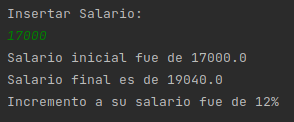
\includegraphics[scale = 1]{images/salario1.png}
	\caption{Output Clase Salario Ejemplo 1}
\end{figure}

\begin{figure}[h]
	\centering
	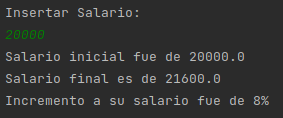
\includegraphics[scale = 1]{images/salario2.png}
	\caption{Output Clase Salario Ejemplo 2}
\end{figure}
\newpage

\begin{figure}[h]
	\centering
	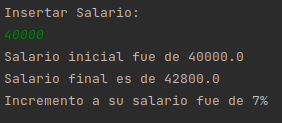
\includegraphics[scale = 1]{images/salario3.png}
	\caption{Output Clase Salario Ejemplo 3}
\end{figure}

\begin{figure}[h]
	\centering
	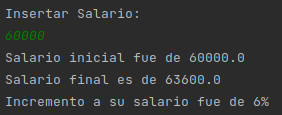
\includegraphics[scale = 1]{images/salario4.png}
	\caption{Output Clase Salario Ejemplo 4}
\end{figure}
\newpage

\subsection{Ejercicio 2}
Escribe un programa en Java que al recibir como datos tres numeors reales, identifique cual es el mayor. Considera que los numeros pueden ser iguales.
Datos: N1, N2 y N3 (variables de tipo real que representan los numeros que se ingresan)\\

\subsubsection{Codigo}

\begin{lstlisting}
import java.util.Scanner;

public class Mayor
{
	public static void main(String[] args)
	{
		Scanner scan = new Scanner(System.in);
		System.out.println("Ingresa numero 1: ");
		float N1 = scan.nextFloat();
		System.out.println("Ingresa numero 2: ");
		float N2 = scan.nextFloat();
		System.out.println("Ingresa numero 3: ");
		float N3 = scan.nextFloat();
		
		float biggest = N1 > N2 ? N1 : N2;
		biggest = biggest > N3 ? biggest : N3;
		
		System.out.println("Numero mayor es: " + biggest);
	}
}
\end{lstlisting}
\newpage
\subsubsection{Evidencias}

\begin{figure}[h]
	\centering
	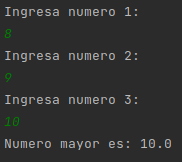
\includegraphics[scale = 1]{images/mayor1.png}
	\caption{Output Clase Mayor Ejemplo 1}
\end{figure}

\begin{figure}[h]
	\centering
	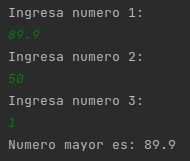
\includegraphics[scale = 1]{images/mayor2.png}
	\caption{Output Clase Mayor Ejemplo 2}
\end{figure}
\newpage

\subsection{Ejercicio 3}

Escribe un programa en Java que permita convertir de pulgadas a milimetros, de yardas a metros y de millas a kilometros.\\

Consideraciones:

\begin{itemize}
	\item 1 pulgada equivale a 25.40 metros
	\item 1 yarda equivale a 0.9144 emtros
	\item 1 milla equivale a 1.6093 kilometros
\end{itemize}

\subsubsection{Codigo}

\begin{lstlisting}
import java.util.Scanner;

public class Converter
{
	public static void main(String[] args)
	{
		Scanner scan = new Scanner(System.in);
		
		System.out.println("Escoja la opcion deseada:");
		System.out.println("1. Pulgadas a Milimetros");
		System.out.println("2. Yardas a Metros");
		System.out.println("3. Millas a Kilometros");
		
		int option = scan.nextInt();
		float data;
		float temp;
		
		switch (option) {
			case 1:
				System.out.println("Indique pulgadas a convertir: ");
				data = scan.nextFloat();
				temp = data;
				data = (float) (data * 25.40);
				System.out.println(temp + " pulgadas, es igual a " + data + " milimetros.");
				break;
				
			case 2:
				System.out.println("Indique yardas a convertir: ");
				data = scan.nextFloat();
				temp = data;
				data = (float) (data * 0.9144);
				System.out.println(temp + " yardas, es igual a " + data + " metros.");
				break;
				
			case 3:
				System.out.println("Indique millas a convertir: ");
				data = scan.nextFloat();
				temp = data;
				data = (float) (data * 1.6093);
				System.out.println(temp + " millas, es igual a " + data + " kilometros.");
				break;
		}
	}
}
\end{lstlisting}
\newpage

\subsubsection{Evidencias}

\begin{figure}[h]
	\centering
	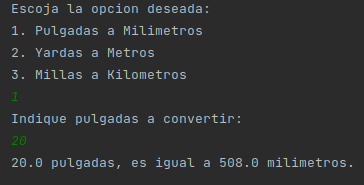
\includegraphics[scale = 0.9]{images/converter1.png}
	\caption{Output Clase Converter Ejemplo 1}
\end{figure}

\begin{figure}[h]
	\centering
	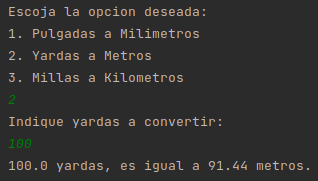
\includegraphics[scale = 1]{images/converter2.png}
	\caption{Output Clase Converter Ejemplo 2}
\end{figure}
\newpage

\begin{figure}[h]
	\centering
	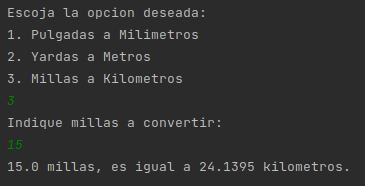
\includegraphics[scale = 1]{images/converter3.png}
	\caption{Output Clase Converter Ejemplo 3}
\end{figure}
\newpage

\subsection{Ejercicio 4}

Escribe un programa en Java al recibir como dato un numero entero N, calcule el resultado de la siguiente serie.\\

$1 + \frac{1}{2} + \frac{1}{3} + \frac{1}{4} + ... + \frac{1}{N}$\\

\subsubsection{Codigo}

\begin{lstlisting}
import java.util.Scanner;

public class Serie
{
	public static void main(String[] args)
	{
		Scanner scan = new Scanner(System.in);
		
		System.out.println("Escoja el denominador limite: ");
		
		int N = scan.nextInt();
		float ans = 0;
		
		for (int i = 1; i <= N; i++)
		{
			ans += 1/(float)i;
		}
		
		System.out.println("El resultado es " + ans);
	}
}
\end{lstlisting}
\newpage

\subsubsection{Evidencias}
\begin{figure}[h]
	\centering
	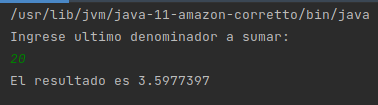
\includegraphics[scale = 1]{images/serie1.png}
	\caption{Output Clase Serie Ejemplo 1}
\end{figure}

\begin{figure}[h]
	\centering
	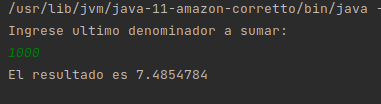
\includegraphics[scale = 1]{images/serie2.png}
	\caption{Output Clase Serie Ejemplo 2}
\end{figure}
\newpage

\subsection{Ejercicio 5}

Escriba una aplicacion que utilice instrucciones de repeticion y switch para imprimir la cancion "Los doce dias de Navidad" (The Twelve Days of Christmas). Una instruccion switch debe utilizarse para imprimir el dia (es decir, first, second, etc).\\

Una instruccion switch separada debe utilizarse para imprimir el resto de cada verso. Visite el sitio (https://es.wikipedia.org/wiki/The\_Twelve\_Days\_of\_Christmas).

\subsubsection{Codigo}

\begin{lstlisting}
public class Christmas
{
	public static void main(String[] args)
	{
		for(int i = 1; i <= 12; i++)
		{
			System.out.print("On the ");
			
			switch(i)
			{
				case 1:
					System.out.print(" first ");
					break;
				case 2:
					System.out.print(" second ");
					break;
				case 3:
					System.out.print(" third ");
					break;
				case 4:
					System.out.print(" fourth ");
					break;
				case 5:
					System.out.print(" fifth ");
					break;
				case 6:
					System.out.print(" sixth ");
					break;
				case 7:
					System.out.print(" seventh ");
					break;
				case 8:
					System.out.print(" eighth");
					break;
				case 9:
					System.out.print(" ninth ");
					break;
				case 10:
					System.out.print(" tenth ");
					break;
				case 11:
					System.out.print(" eleventh ");
					break;
				case 12:
					System.out.print(" twelfth");
					break;
			}
			
			System.out.println(" day of Christmas, my true love sent to me");
			
			for(int k = i; k >= 0; k--)
			{
				switch(k)
				{
					case 1:
						if(i > 1)
						{
							System.out.print("and ");
						}
						System.out.println("a Partridge in a Pear Tree.");
						break;
					case 2:
						System.out.println("Two turtle doves,");
						break;
					case 3:
						System.out.println("Three french hens,");
						break;
					case 4:
						System.out.println("Four calling birds,");
						break;
					case 5:
						System.out.println("Five golden rings,");
						break;
					case 6:
						System.out.println("Six geese a-laying,");
						break;
					case 7:
						System.out.println("Seven swans a-swimming,");
						break;
					case 8:
						System.out.println("Eight maids a-milking,");
						break;
					case 9:
						System.out.println("Nine ladies dancing,");
						break;
					case 10:
						System.out.println("Ten lords a-leaping,");
						break;
					case 11:
						System.out.println("Eleven pipers piping,");
						break;
					case 12:
						System.out.println("Twelve drummers drumming,");
						break;
				}
			}
			System.out.println();
		}
	}
}
\end{lstlisting}
\newpage

\subsubsection{Evidencias}

\begin{figure}[H]
	\centering
	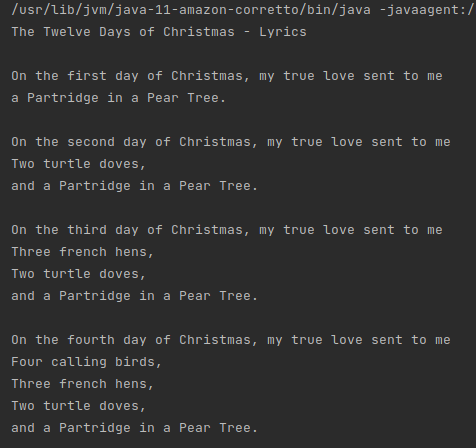
\includegraphics[scale = 0.8]{images/xmas1.png}
	\caption{Output Clase Christmas Ejemplo 1}
\end{figure}

\begin{figure}[H]
	\centering
	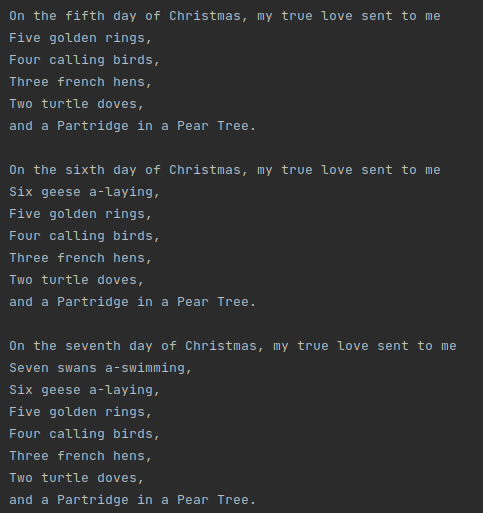
\includegraphics[scale = 0.8]{images/xmas2.png}
	\caption{Output Clase Christmas Ejemplo 2}
\end{figure}

\begin{figure}[H]
	\centering
	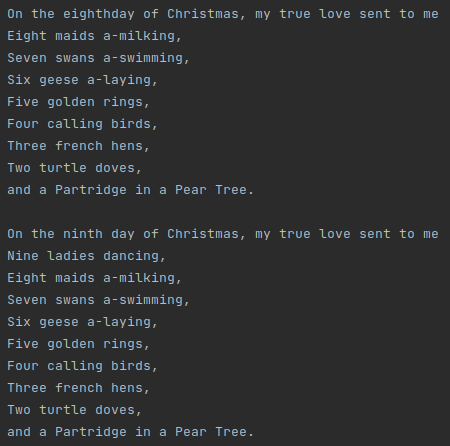
\includegraphics[scale = 0.8]{images/xmas3.png}
	\caption{Output Clase Christmas Ejemplo 3}
\end{figure}

\begin{figure}[H]
	\centering
	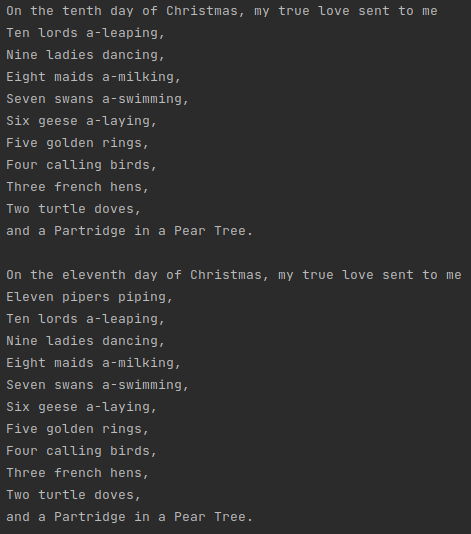
\includegraphics[scale = 0.8]{images/xmas4.png}
	\caption{Output Clase Christmas Ejemplo 4}
\end{figure}

\begin{figure}[H]
	\centering
	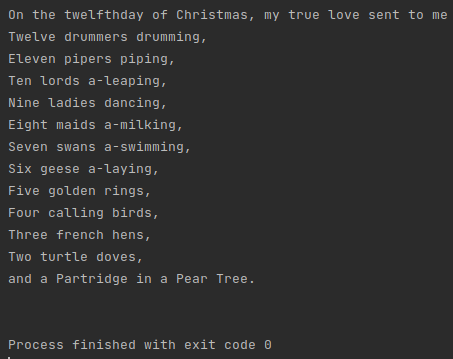
\includegraphics[scale = 0.8]{images/xmas5.png}
	\caption{Output Clase Christmas Ejemplo 5}
\end{figure}
\newpage
\section{Conclusiones}

Durante esta practica me gusto hacerla pues no se me hizo tan complicado a excepcion del ultimo ejercicio que estuvo un poco "tricky", pero al final me salio muy bien. En realidad algo que me doy cuenta, es que en general, los lenguajes de programacion no difieren mucho unos de los otros, pues la mayoria estan relacionados en cuanto a los usos de las estructuras de control, loops, tipos de datos primitivos, etc.\\

La unica cosa en la que por lo regular cambian los lenguajes es en su sintaxis en ocasiones y el paradigma que presentan.\\

Uno de los principales cambios con respecto de este lenguaje Java que si me llamo la atencion es la parte de los objetos, pues aun me estoy familiriazando con el tema. Tambien la parte de los "getters" y "setters" aunque aun no la comprendo del todo, me parece que es casi una funcion para cada una de las variables en vez de poder hacer una para todas. Aunque aun no entiendo del todo como funcionan apropiadamente,\\ 

En general la practica no se me hizo del todo complicada y me parece que quedo muy bien.\\

Gracias por leer mi practica.


\end{document}